\subsection{Hom関手}\label{chap-6.4-hom-functor}
  いよいよ射集合を取る操作が関手であることを示そう。その前に射写像を取る操作が関手の性質を満たすことを先に示しておく。
	\begin{prop}[共変射写像の恒等射の保存]\label{prop-preservation-identity-arrow-by-covariant-arrow-map}
		圏$\cat{C}$の任意の対象$X,A$において
		\[\arset{C}{X}{id_A}=id_{\arset{C}{X}{A}}\]が成り立つ。
		\begin{center}
			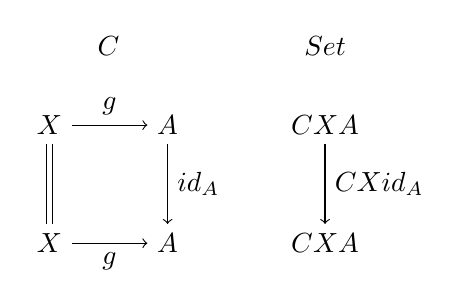
\begin{tikzpicture}[auto]
				\node (x) at (-1.5, 0) {$X$};
				\node (x2) at (-1.5, -1.5) {$X$};
				\node (a) at (0, 0) {$A$};
				\node (b) at (0, -1.5) {$A$};
				\node (ca) at (2, 0) {$\arset{C}{X}{A}$};
				\node (cb) at (2, -1.5) {$\arset{C}{X}{A}$};
				\node (catc) at (-0.75, 1) {$\cat{C}$};
				\node (catc) at (2, 1) {$\cat{Set}$};
				\draw[->] (ca) to node{$\arset{C}{X}{id_A}$}(cb);
				\draw[->] (a) to node{$id_A$}(b);
				\draw[double distance=2pt] (x) to (x2);
				\draw[->] (x) to node{$g$}(a);
				\draw[->] (x2) to node[swap]{$g$}(b);
			\end{tikzpicture}
		\end{center}
	\end{prop}
	\begin{proof}
		任意の射$\mor{g}{X}{A}$に対して
		\begin{align*}
			\arset{C}{X}{id_A}(g)&=id_A\circ g&\text{(共変射写像の定義)}\\
			&=g&\text{(単位元律)}\\
			&=id_{\arset{C}{X}{A}}(g)&\text{($\cat{Set}$の恒等射の定義)}\\
		\end{align*}
		よって$\arset{C}{X}{id_A}=id_{\arset{C}{X}{A}}$が成り立つ。
	\end{proof}
	\begin{prop}[共変射写像の合成の保存]\label{prop-preservation-composition-by-covariant-arrow-map}
		圏$\cat{C}$の任意の対象$X,A,B,C$と射$\mor{f}{A}{B}$、$\mor{g}{B}{C}$、$\mor{h}{X}{A}$に対して、
		\[\arset{C}{X}{g\circ f}=\arset{C}{X}{g}\circ\arset{C}{X}{f}\]が成り立つ。
		\begin{center}
			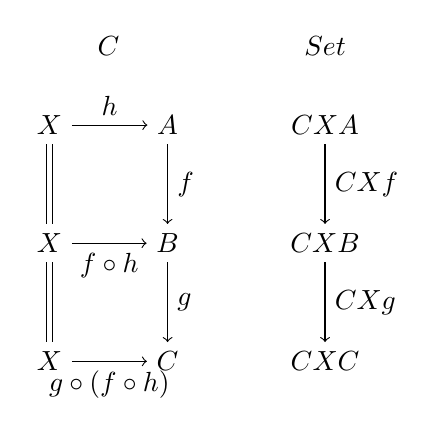
\begin{tikzpicture}[auto]
				\node (x) at (-1.5, 0) {$X$};
				\node (x2) at (-1.5, -1.5) {$X$};
				\node (x3) at (-1.5, -3) {$X$};
				\node (a) at (0, 0) {$A$};
				\node (b) at (0, -1.5) {$B$};
				\node (c) at (0, -3) {$C$};
				\node (ca) at (2, 0) {$\arset{C}{X}{A}$};
				\node (cb) at (2, -1.5) {$\arset{C}{X}{B}$};
				\node (cc) at (2, -3) {$\arset{C}{X}{C}$};
				\node (catc) at (-0.75, 1) {$\cat{C}$};
				\node (catc) at (2, 1) {$\cat{Set}$};
				\draw[->] (ca) to node{$\arset{C}{X}{f}$}(cb);
				\draw[->] (cb) to node{$\arset{C}{X}{g}$}(cc);
				\draw[->] (a) to node{$f$}(b);
				\draw[->] (b) to node{$g$}(c);
				\draw[double distance=2pt] (x) to (x2);
				\draw[double distance=2pt] (x2) to (x3);
				\draw[->] (x) to node{$h$}(a);
				\draw[->] (x2) to node[swap]{$f\circ h$}(b);
				\draw[->] (x3) to node[swap]{$g\circ(f\circ h)$}(c);
			\end{tikzpicture}
		\end{center}
	\end{prop}
	\begin{proof}
		任意の射$\mor{h}{X}{A}$に対して
		\begin{align*}
			\arset{C}{X}{g\circ f}(h)&=(g\circ f)\circ h&\text{(共変射関数の定義)}\\
			&=g\circ(f\circ h)&\text{(結合則)}\\
			&=\arset{C}{X}{g}(f\circ h)&\text{(共変射関数の定義)}\\
			&=\arset{C}{X}{g}(\arset{C}{X}{f}(h))&\text{(共変射関数の定義)}\\
			&=\arset{C}{X}{g}\circ\arset{C}{X}{f}(h)&\text{(写像の合成の定義)}\\
		\end{align*}
		よって$\arset{C}{X}{g\circ f}=\arset{C}{X}{g}\circ\arset{C}{X}{f}$が成り立つ。
	\end{proof}
	\begin{define}[共変Hom関手]\label{def-covariant-hom-functor}
		任意の圏$\cat{C}$とそのある対象$X$における共変Hom関手$\functor{\arset{C}{X}{-}}{C}{Set}$を以下の要素で定義する。
		\begin{quote}
			\begin{mydescription}
				\item[対象関数] 圏$\cat{C}$の任意の対象$A$に対して対象関数を
				\begin{align*}
					&\mor{\arset{C}{X}{-}}{\obj{C}}{\obj{Set}}\\
					&\arset{C}{X}{-}(A)=\arset{C}{X}{A}
				\end{align*}
				と定義する。
				\item[射関数] 圏$\cat{C}$の任意の対象$A,B$、射$\mor{f}{A}{B}$に対して射関数を
				\begin{align*}
					&\mor{\arset{C}{X}{-}_{A,B}}{\arset{C}{A}{B}}{\arset{Set}{\arset{C}{X}{A}}{\arset{C}{X}{B}}}\\
					&\arset{C}{X}{-}_{A,B}(f)=\arset{C}{X}{f}
				\end{align*}
				と定義する。
				\begin{center}
					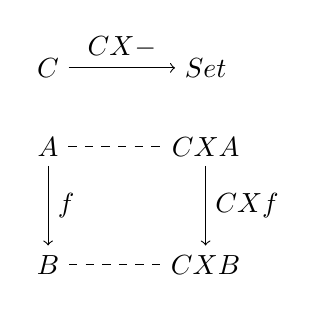
\begin{tikzpicture}[auto]
						\node (a) at (0, 0) {$A$};
						\node (b) at (0, -1.5) {$B$};
						\node (ca) at (2, 0) {$\arset{C}{X}{A}$};
						\node (cb) at (2, -1.5) {$\arset{C}{X}{B}$};
						\node (catc) at (0, 1) {$\cat{C}$};
						\node (catset) at (2, 1) {$\cat{Set}$};
						\draw[->] (ca) to node{$\arset{C}{X}{f}$}(cb);
						\draw[->] (a) to node{$f$}(b);
						\draw[->] (catc) to node{$\arset{C}{X}{-}$}(catset);
						\draw[-,dashed] (a) to (ca);
						\draw[-,dashed] (b) to (cb);
					\end{tikzpicture}
				\end{center}
				\item[恒等射の保存] 共変射写像の合成の保存より、$\arset{C}{X}{id_A}=id_{\arset{C}{X}{A}}$が成り立つ。
				\item[射の合成の保存] 共変射写像の恒等射の保存より、$\arset{C}{X}{g\circ f}=\arset{C}{X}{g}\circ\arset{C}{X}{f}$が成り立つ。
			\end{mydescription}
		\end{quote}
	\end{define}
	
	また反変射写像をとる操作を射関数とした関手は反変関手として定義する。
		\begin{define}[反変Hom関手]\label{def-contravariant-hom-functor}
		任意の圏$\cat{C}$とそのある対象$X$における反変Hom関手$\functor{\arset{C}{X}{-}}{C^{op}}{Set}$を以下の要素で定義する。
		\begin{quote}
			\begin{mydescription}
				\item[対象関数] 圏$\cat{C}$の任意の対象$A$に対して対象関数を
				\begin{align*}
					&\mor{\arset{C}{-}{X}}{\obj{C}}{\obj{Set}}\\
					&\arset{C}{-}{X}(A)=\arset{C}{X}{A}
				\end{align*}
				と定義する。
				\item[射関数] 圏$\cat{C}$の任意の対象$A,B$、射$\mor{f}{A}{B}$に対して射関数を
				\begin{align*}
					&\mor{\arset{C}{-}{X}_{A,B}}{\arset{C}{A}{B}}{\arset{Set}{\arset{C}{B}{X}}{\arset{C}{A}{X}}}\\
					&\arset{C}{-}{X}_{A,B}(f)=\arset{C}{f}{X}
				\end{align*}
				と定義する。
				\begin{center}
					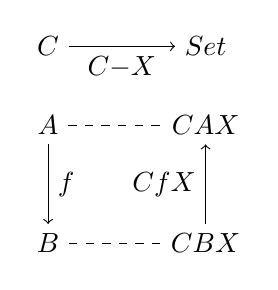
\begin{tikzpicture}[auto]
						\node (a) at (0, 0) {$A$};
						\node (b) at (0, -1.5) {$B$};
						\node (ca) at (2, 0) {$\arset{C}{A}{X}$};
						\node (cb) at (2, -1.5) {$\arset{C}{B}{X}$};
						\node (catc) at (0, 1) {$\cat{C}$};
						\node (catset) at (2, 1) {$\cat{Set}$};
						\draw[->] (cb) to node{$\arset{C}{f}{X}$}(ca);
						\draw[->] (a) to node{$f$}(b);
						\draw[->] (catc) to node[swap]{$\arset{C}{-}{X}$}(catset);
						\draw[-,dashed] (a) to (ca);
						\draw[-,dashed] (b) to (cb);
					\end{tikzpicture}
				\end{center}
				\item[恒等射の保存] 共変射写像の合成の保存と同様に$\arset{C}{id_A}{X}=id_{\arset{C}{A}{X}}$が成り立つ。
				\item[射の合成の保存] 共変射写像の恒等射の保存と同様に$\arset{C}{g\circ f}{X}=\arset{C}{f}{X}\circ\arset{C}{g}{X}$が成り立つ。
			\end{mydescription}
		\end{quote}
	\end{define}
  さて射集合、射写像を取る操作が関手であることを示せたから、これらが関手としてどのような性質をもつのか少し確認する。
	\begin{prop}[Hom関手の積の保存]\label{prop-preservation-product-by-hom-functor}
		圏$\cat{C}$の積$A\times B$に対して、\[\arset{C}{X}{A\times B}\cong \arset{C}{X}{A}\times \arset{C}{X}{B}\]が成り立つ。
	\end{prop}
	\begin{proof}
		$\arset{C}{X}{A}\times\arset{C}{X}{B}$は$\arset{C}{X}{A}$と$\arset{C}{X}{B}$の積であるが、$\arset{C}{X}{A\times B}$も同様に$\arset{C}{X}{A}$と$\arset{C}{X}{B}$の積であることを示せばよい。
		射影射をそれぞれ
		\begin{align*}
			&\pi_{\arset{C}{X}{A}}=\mor{\arset{C}{X}{\pi_A}}{\arset{C}{X}{A\times B}}{\arset{C}{X}{A}}\\
			&\pi_{\arset{C}{X}{B}}=\mor{\arset{C}{X}{\pi_B}}{\arset{C}{X}{A\times B}}{\arset{C}{X}{B}}
		\end{align*}
		として、組$(\arset{C}{X}{A\times B},\arset{C}{X}{\pi_A},\arset{C}{X}{\pi_B})$が積の普遍性を満たすことを証明する。つまり$\cat{Set}$の任意の対象$Y$と任意の二射$\mor{i}{Y}{\arset{C}{X}{A}}$、$\mor{j}{Y}{\arset{C}{X}{B}}$に対して、
		\begin{align*}
			&\arset{C}{X}{\pi_A}\circ\tuple{i,j}=i\\
			&\arset{C}{X}{\pi_B}\circ\tuple{i,j}=j
		\end{align*}
		が成り立つような射$\mor{\tuple{i,j}}{Y}{\arset{C}{X}{A\times B}}$が一意に存在することを示せばよい。\\
    証明の方向性としては集合の圏$\cat{Set}$の射\[\mor{i}{Y}{\arset{C}{X}{A}},\ \mor{j}{Y}{\arset{C}{X}{A}}\]に$Y$の元$y$を適用すると、圏$\cat{C}$の射\[\mor{i(y)}{X}{A},\ \mor{j(y)}{X}{B}\]が得られるが、集合の圏$\cat{Set}$の射の対$\tuple{i,j}$の存在と一意性を、圏$\cat{C}$の積の普遍性で示すことで証明する。\\
		まずは図式を可換にする$\tuple{i,j}$を定義し、常に存在することを示す。
		\begin{center}
			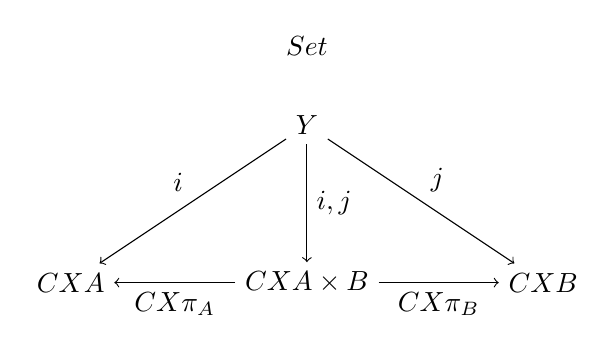
\begin{tikzpicture}[auto]
				\node (set) at (3, 3) {$\cat{Set}$};
				\node (xa) at (0, 0) {$\arset{C}{X}{A}$};
				\node (xab) at (3, 0) {$\arset{C}{X}{A\times B}$};
				\node (xb) at (6, 0) {$\arset{C}{X}{B}$};
				\node (y) at (3, 2) {$Y$};
				\draw[->] (xab) to node{$\arset{C}{X}{\pi_A}$}(xa);
				\draw[->] (xab) to node[swap]{$\arset{C}{X}{\pi_B}$}(xb);
				\draw[->] (y) to node[swap]{$i$}(xa);
				\draw[->] (y) to node{$j$}(xb);
				\draw[->] (y) to node{$\tuple{i,j}$}(xab);
			\end{tikzpicture}
		\end{center}
		ここで対象$Y$の任意の元$y$を取り適用すると、圏$\cat{C}$の射$\mor{i(y)}{X}{A}$、$\mor{j(y)}{X}{B}$が得られる。

		射$i,j$は$\cat{Set}$の射であるが、値を適用した$i(y),j(y)$もまた$\cat{C}$の射であることに注意してほしい。もし圏$\cat{C}$で対象$X$の元$x$が取れるなら、さらに値を適用して対象$A$の元$i(y)(x)$が取れる。

		圏$\cat{C}$の積$(A\times B,\pi_A,\pi_B)$に対して射$i(y),j(y)$の射の対\[\mor{\tuple{i(y),j(y)}}{X}{A\times B}\]を考える。
		\begin{center}
			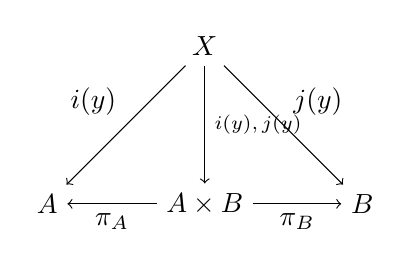
\begin{tikzpicture}[auto]
				\node (a) at (0, 0) {$A$};
				\node (b) at (4, 0) {$B$};
				\node (ab) at (2, 0) {$A\times B$};
				\node (x) at (2, 2) {$X$};
				\draw[->] (ab) to node {$\pi_A$}(a);
				\draw[->] (ab) to node[swap] {$\pi_B$}(b);
				\draw[->] (x) to node[swap] {$i(y)$}(a);
				\draw[->] (x) to node {$j(y)$}(b);
				\draw[->] (x) to node {\scriptsize{$\tuple{i(y),j(y)}$}}(ab);
			\end{tikzpicture}
		\end{center}
		このような射の対は任意の射$i(y),j(y)$に対して存在するから、任意の$y$に対しても存在する。
		よって$\cat{Set}$の射の対$\tuple{i,j}$を任意の$y$に対して\[\tuple{i,j}(y)=\tuple{i(y),j(y)}\]と定義できた。
		次に$\tuple{i,j}$が図式を可換にすることを示す。

		同様に$Y$の任意の元$y$に対し
		\begin{align*}
			\arset{C}{X}{\pi_A}\circ\tuple{i,j}(y)&=\arset{C}{X}{\pi_A}(\tuple{i,j}(y))&\text{(射の合成の定義)}\\
			&=\arset{C}{X}{\pi_A}(\tuple{i(y),j(y)})&\text{($\tuple{i,j}$の定義)}\\
			&=\pi_A\circ(\tuple{i(y),j(y)})&\text{(共変射写像の定義)}\\
			&=i(y)&\text{(射の対の可換性)}
		\end{align*}
		よって$\arset{C}{X}{\pi_A}\circ\tuple{i,j}=i$が成り立つ。同様に$\arset{C}{X}{\pi_B}\circ\tuple{i,j}=j$も成り立つ。

		次に射の対$\tuple{i,j}$の一意性を示す。
		ある射$\mor{k}{Y}{\arset{C}{X}{A\times B}}$が
		\begin{align*}
			&\arset{C}{X}{\pi_A}\circ k=i\\
			&\arset{C}{X}{\pi_B}\circ k=j
		\end{align*}
		を満たすとき、$h=\tuple{i,j}$が成り立つことを示せばよい。

		$Y$の任意の元$y$に対し
		\begin{align*}
			i(y)&=(\arset{C}{X}{\pi_A}\circ k)(y)\\
			&=\arset{C}{X}{\pi_A}(k(y))&\text{(射の合成の定義)}\\
			&=\pi_A\circ(k(y))&\text{(共変射写像の定義)}
		\end{align*}
		よって$\pi_A\circ(k(y))=i(y)$が成り立つ。同様に$\pi_A\circ(k(y))=i(y)$も成り立つ。
		すると$\cat{C}$の積$A\times B$の射の対$\tuple{i,j}(y)$の一意性より、$k(y)=\tuple{i,j}(y)$となる。
		これは任意の$y$で成り立つから$k=\tuple{i,j}$となり、$\tuple{i,j}$は$i,j$に対して一意に存在することが示せた。
		\begin{center}
			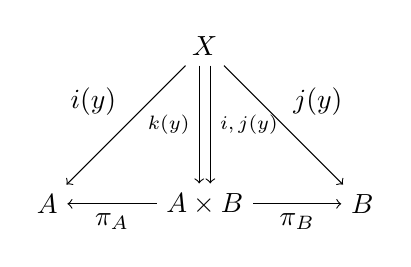
\begin{tikzpicture}[auto]
				\node (a) at (0, 0) {$A$};
				\node (b) at (4, 0) {$B$};
				\node (ab) at (2, 0) {$A\times B$};
				\node (x) at (2, 2) {$X$};
				\draw[->] (ab) to node {$\pi_A$}(a);
				\draw[->] (ab) to node[swap] {$\pi_B$}(b);
				\draw[->] (x) to node[swap] {$i(y)$}(a);
				\draw[->] (x) to node {$j(y)$}(b);
				\draw[->,transform canvas={xshift=+2pt}] (x) to node {\scriptsize{$\tuple{i,j}(y)$}}(ab);
				\draw[->,transform canvas={xshift=-2pt}] (x) to node[swap] {\scriptsize{$k(y)$}}(ab);
			\end{tikzpicture}
		\end{center}
		よって組$(\arset{C}{X}{A\times B},\arset{C}{X}{\pi_A},\arset{C}{X}{\pi_B})$は積の普遍性を満たす。つまり$\arset{C}{X}{A\times B}$は$\arset{C}{X}{A}$と$\arset{C}{X}{B}$の積であり、積の一意性より、\[\arset{C}{X}{A\times B}\cong \arset{C}{X}{A}\times \arset{C}{X}{B}\]が成り立つ。
	\end{proof}
	かなり長い証明になってしまったが、$\arset{C}{X}{A\times B}\cong \arset{C}{X}{A}\times \arset{C}{X}{B}$を示すだけなら同型射となるような射を定義して同型射であることを証明すればよい。こちらの方が簡単ではあるが、同型射を射集合を用いた議論に慣れてもらうためこのように証明した。

	さてこの同型の意味を考えると、任意の二射$\mor{f}{X}{A}$、$\mor{g}{X}{B}$と射の対$\mor{\tuple{f,g}}{X}{A\times B}$が一対一対応をする、ということになる。ただし現段階では逆は成り立たない。

  また、証明中では特に区別しなかったが、集合の圏の積による射の対を$\mor{[f,g]}{1}{\arset{C}{X}{A}\times\arset{C}{X}{B}}$、圏$\cat{C}$の積による射の対を$\mor{\tuple{f,g}}{X}{A\times B}$として、同型射をそれぞれ、\[\mor{i}{\arset{C}{X}{A\times B}}{\arset{C}{X}{A}\times\arset{C}{X}{B}}\]\[\mor{i^{-1}}{\arset{C}{X}{A}\times\arset{C}{X}{B}}{\arset{C}{X}{A\times B}}\]とすると、\[i(\tuple{f,g})=[f,g],\ i^{-1}([f,g])=\tuple{f,g}\]となる射であることが、積の一意性の証明から分かる。
  つまり、これらの同型射は、圏$\cat{C}$の射の対と集合の圏の射の対を相互に変換する写像であることが分かる。


  これらの射が既存の射を用いてどのように構成されるかを示したいところではあるが、射の対の種類が更に増えてややこしくなってしまうため、ここでは結果だけを示した。

	次に自明ではあるが、共変Hom関手が終対象を保つことを同様に証明する。
	\begin{prop}[Hom関手の終対象の保存]\label{prop-preservation-terminal-object-by-hom-functor}
		圏$\cat{C}$の終対象$1$と圏$\cat{Set}$の任意の対象$X$と終対象$I$に対して\[\arset{C}{X}{1}\cong I\]が成り立つ。
	\end{prop}
	\begin{proof}
		$\arset{C}{X}{1}$が$\cat{Set}$における終対象であることを示せばよい。つまり$\cat{Set}$の任意の対象$Y$に対して\[\mor{!_Y}{Y}{\arset{C}{X}{1}}\]が一意に存在することを証明する。

		射$\mor{!_Y}{Y}{\arset{C}{X}{1}}$が少なくとも一つは存在すると仮定する。
		対象$Y$の任意の元$y$を$!_Y$に適用すると圏$\cat{C}$の射$\mor{!_Y(y)}{X}{1}$が得られるが、終対象$1$の普遍性よりこのような射は少なくとも一つは存在する。よって任意の$y$において$!_Y(y)$が存在するから、実際に射$!_Y$は存在する。
		\begin{center}
			\begin{tikzpicture}[auto]
				\node (set) at (1, 1) {$\cat{Set}$};
				\node (1) at (0, 0) {$Y$};
				\node (1') at (2, 0) {$\arset{C}{X}{1}$};
				\node (set) at (5, 1) {$\cat{C}$};
				\node (x) at (4, 0) {$X$};
				\node (t) at (6, 0) {$1$};
				\draw[->] (1) to node{$!_Y$}(1');
				\draw[->] (x) to node{$!_Y(y)$}(t);
			\end{tikzpicture}
		\end{center}
		次に$\mor{!_Y}{Y}{\arset{C}{X}{1}}$の一意性を示す。つまり射$\mor{h}{Y}{\arset{C}{X}{1}}$が存在したとき、$!_Y=h$が成り立てばよい。

		対象$Y$の任意の元$y$において射$\mor{h(y)}{X}{1}$に対して圏$\cat{C}$の終対象の普遍性より、$\mor{!_Y(y)}{X}{1}$なる射は一意に存在する。よって$!_Y(y)=h(y)$となり、任意の元$y$で成り立つから$!_Y=h$となる。

		\begin{center}
			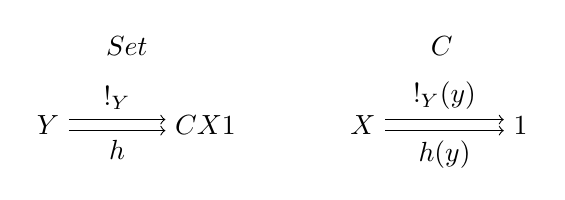
\begin{tikzpicture}[auto]
				\node (set) at (1, 1) {$\cat{Set}$};
				\node (1) at (0, 0) {$Y$};
				\node (1') at (2, 0) {$\arset{C}{X}{1}$};
				\node (set) at (5, 1) {$\cat{C}$};
				\node (x) at (4, 0) {$X$};
				\node (t) at (6, 0) {$1$};
				\draw[->,transform canvas={yshift=2pt}] (1) to node{$!_Y$}(1');
				\draw[->,transform canvas={yshift=2pt}] (x) to node{$!_Y(y)$}(t);
				\draw[->,transform canvas={yshift=-2pt}] (1) to node[swap]{$h$}(1');
				\draw[->,transform canvas={yshift=-2pt}] (x) to node[swap]{$h(y)$}(t);
			\end{tikzpicture}
		\end{center}
		$\mor{!_Y}{Y}{\arset{C}{X}{1}}$なる射が一意に存在することが示せたから、$\arset{C}{X}{1}$は$\cat{Set}$における終対象となる。よって終対象の一意性より、\[\arset{C}{X}{1}\cong I\]が成り立つ。
	\end{proof}

	次に積関手を双積関手に一般化したように、共変Hom関手、反変Hom関手を双関手として定義する。
	\begin{define}[双Hom関手]\label{def-dihom-functor}
		任意の圏$\cat{C}$における\textbf{双Hom関手}$\functor{C(-,-)}{C^{op}\times C}{Set}$を以下の要素で定義する。
		\begin{quote}
			\begin{mydescription}
				\item[対象関数] 積圏$\cat{C^{op}\times C}$の任意の対象$[A,B]$に対して対象関数を
				\begin{align*}
					&\mor{\arset{C}{-}{-}}{\obj{C^{op}\times C}}{\obj{Set}}\\
					&\arset{C}{-}{-}([A,B])=\arset{C}{A}{B}
				\end{align*}
				と定義する。
				\item[射関数]射関数を定義する前に共変射写像、反変射写像の双Hom関手版を定義する。
				圏$\cat{C^{op}}$の任意の射$\mor{f^{op}}{A^{op}}{A'^{op}}$、つまり圏$\cat{C}$の射$\mor{f}{A'}{A}$と圏$\cat{C}$の任意の射$\mor{g}{B}{B'}$に対し射写像\[\mor{\arset{C}{f}{g}}{\arset{C}{A}{B}}{\arset{C}{A'}{B'}}\]を任意の射$\mor{h}{A}{B}$において、
				\begin{align*}
					\arset{C}{f}{g}&=\arset{C}{f}{B'}\circ\arset{C}{A}{g}\\
					&=\arset{C}{A'}{g}\circ\arset{C}{f}{B}\\
					\arset{C}{f}{g}(h)&=g\circ h\circ f\\
				\end{align*}
				と定義する。

				\begin{center}
					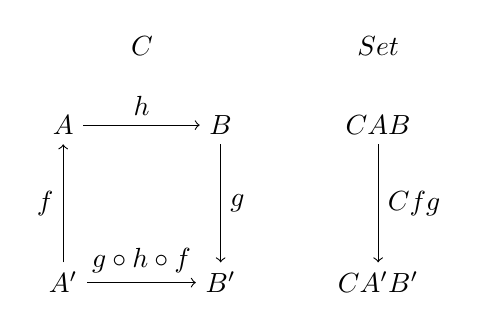
\begin{tikzpicture}[auto]
						\node (A) at (0, 0) {$A$};
						\node (A') at (0, -2) {$A'$};
						\node (B) at (2, 0) {$B$};
						\node (B') at (2, -2) {$B'$};
						\draw[->] (A') to node{$f$}(A);
						\draw[->] (B) to node{$g$}(B');
						\draw[->] (A) to node{$h$}(B);
						\draw[->] (A') to node{$g\circ h\circ f$}(B');
						\node (AB) at (4, 0) {$\arset{C}{A}{B}$};
						\node (A'B') at (4, -2) {$\arset{C}{A'}{B'}$};
						\draw[->] (AB) to node{$\arset{C}{f}{g}$}(A'B');
						\node (catc) at (1, 1) {$\cat{C}$};
						\node (catset) at (4, 1) {$\cat{Set}$};
					\end{tikzpicture}
				\end{center}

				圏$\cat{C^{op}\times C}$の任意の対象$[A,B],[A',B']$、射$\mor{f}{A}{B}$に対して射関数を
				\begin{align*}
					&\mor{\arset{C}{-}{-}}{\arset{(C^{op}\times C)}{[A,B]}{[A',B']}}{\arset{Set}{\arset{C}{A}{B}}{\arset{C}{A'}{B'}}}\\
					&\arset{C}{-}{-}([f,g])=\arset{C}{f}{g}
				\end{align*}
				と定義する。
				\begin{center}
					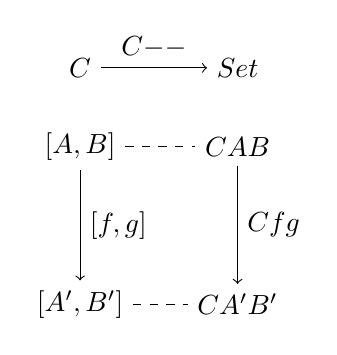
\begin{tikzpicture}[auto]
						\node (ab) at (0, 0) {$[A,B]$};
						\node (a'b') at (0, -2) {$[A',B']$};
						\draw[->] (ab) to node{$[f,g]$}(a'b');
						\node (sab) at (2, 0) {$\arset{C}{A}{B}$};
						\node (sa'b') at (2, -2) {$\arset{C}{A'}{B'}$};
						\draw[->] (sab) to node{$\arset{C}{f}{g}$}(sa'b');
						\draw[-,dashed] (ab) to (sab);
						\draw[-,dashed] (a'b') to (sa'b');
						\node (catc) at (0, 1) {$\cat{C}$};
						\node (catset) at (2, 1) {$\cat{Set}$};
						\draw[->] (catc) to node{$\arset{C}{-}{-}$}(catset);
					\end{tikzpicture}
				\end{center}
				\item[恒等射の保存] 圏$\cat{C^{op}\times C}$の任意の対象$[A,B]$に対して\[\arset{C}{-}{-}(id_{[A,B]})=\mor{id_{\arset{C}{-}{-}([A,B])}}{\arset{C}{A}{B}}{\arset{C}{A}{B}}\]を示せばよい。

				任意の積圏の射$\mor{f}{A}{B}$に対して
				\begin{align*}
					\arset{C}{-}{-}(id_{[A,B]})(f)&=\arset{C}{-}{-}([id_A,id_B])(f)&\text{(積圏の恒等射の定義)}\\
					&=\arset{C}{id_A}{id_B}(f)&\text{(対象関数の定義)}\\
					&=id_B\circ f\circ id_A&\text{(射写像の定義)}\\
					&=f&\text{(圏$\cat{C}$の単位元律)}\\
					&=id_{\arset{C}{A}{B}}(f)&\text{($\cat{Set}$の単位元律)}\\
					&=id_{\arset{C}{-}{-}([A,B])}(f)&\text{(対象関数の定義)}
				\end{align*}
				よって$\arset{C}{-}{-}(id_{[A,B]})=id_{\arset{C}{-}{-}([A,B])}$が成り立ち恒等射の保存が成り立つ。


				\item[射の合成の保存] $\cat{Set}$の任意の射写像$\mor{\arset{C}{f}{g}}{\arset{C}{A}{B}}{\arset{C}{A'}{B'}}$、$\mor{\arset{C}{f'}{g'}}{\arset{C}{A'}{B'}}{\arset{C}{A''}{B''}}$に対して\[\arset{C}{f'}{g'}\circ\arset{C}{f}{g}=\arset{C}{f\circ f'}{g'\circ g}\]が成り立てばよい。

				圏$\cat{C}$の任意の射$\mor{h}{A}{B}$に対して
				\begin{align*}
					(\arset{C}{f'}{g'}\circ\arset{C}{f}{g})(h)&=(\arset{C}{f'}{g'})(g\circ h\circ f)&\text{(射写像の定義)}\\
					&=g'\circ(g\circ h\circ f)\circ f'&\text{(射写像の定義)}\\
					&=(g'\circ g)\circ h\circ(f\circ f')&\text{(結合律)}\\
					&=\arset{C}{f\circ f'}{g'\circ g}(h)&\text{(射写像の定義)}\\
				\end{align*}
				よって$\arset{C}{f'}{g'}\circ\arset{C}{f}{g}=\arset{C}{f\circ f'}{g'\circ g}$となり射の合成の保存が成り立つ。
			\end{mydescription}
		\end{quote}
	\end{define}

	双積関手、双Hom関手を定義したときは完全に新しい関手として対象関数、射関数から定義した。しかし、これらの例のように、右側と左側の関手がそれぞれ定まっていて、ある条件を満たしていれば二つの関手から双関手を定義できる。\\メリットとしてこの定義を用いれば双関手の恒等射の保存と合成の保存を個別に証明しなくても済む。
	\begin{define}[二つの関手による双関手の定義]\label{def-bifunctor-by-two-functors}
		圏$\cat{B}$の任意の対象$B$に対して定義される関手$\functor{F_B}{A}{C}$と、圏$\cat{A}$の任意の対象$A$に対して定義される関手$\functor{G_A}{B}{C}$が存在し、任意の二対象$A,B$に対して\[{F_B}A={G_A}B\]が成り立ち、	任意の二射$\mor{f}{A}{A'}$、$\mor{g}{B}{B'}$に対して\[{G_{A'}}g\circ {F_B}f = {F_{B'}}f\circ {G_A}g\]が成り立つとする。
		\begin{center}
			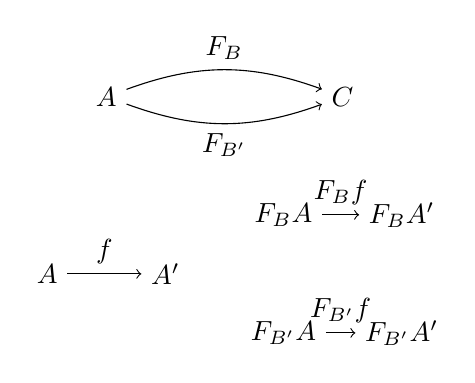
\begin{tikzpicture}[auto]
				\node (A) at (0, 0.75) {$A$};
				\node (B) at (1.5, 0.75) {$A'$};
				\node (FA) at (3, 1.5) {${F_B}A$};
				\node (FB) at (4.5, 1.5) {${F_B}A'$};
				\node (GA) at (3, 0) {${F_{B'}}A$};
				\node (GB) at (4.5, 0) {${F_{B'}}A'$};

				\node (catc) at (0.75, 3) {$\cat{A}$};
				\node (catd) at (3.75, 3) {$\cat{C}$};

				\draw[->] (A) to node{$f$}(B);
				\draw[->] (FA) to node{${F_B}f$}(FB);
				\draw[->] (GA) to node{${F_{B'}}f$}(GB);
				\draw[->,bend left = 20] (catc) to node (funcf){$F_B$}(catd);
				\draw[->,bend right = 20] (catc) to node (funcg)[swap]{$F_{B'}$}(catd);
			\end{tikzpicture}
			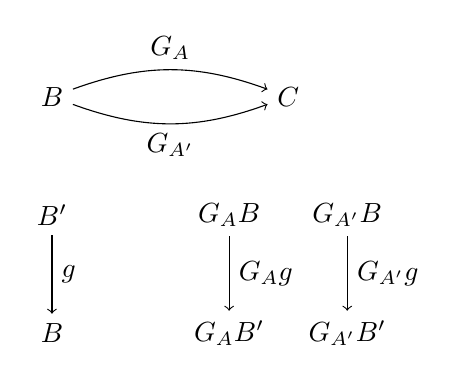
\begin{tikzpicture}[auto]
				\node (A) at (0.75, 0) {$B$};
				\node (B) at (0.75, 1.5) {$B'$};
				\node (FA) at (3, 1.5) {${G_A}B$};
				\node (FB) at (4.5, 1.5) {${G_{A'}}B$};
				\node (GA) at (3, 0) {${G_{A}}B'$};
				\node (GB) at (4.5, 0) {${G_{A'}}B'$};

				\node (catc) at (0.75, 3) {$\cat{B}$};
				\node (catd) at (3.75, 3) {$\cat{C}$};

				\draw[->] (B) to node{$g$}(A);
				\draw[->] (FA) to node{${G_A}g$}(GA);
				\draw[->] (FB) to node{${G_{A'}}g$}(GB);

				\draw[->,bend left = 20] (catc) to node (funcf){$G_A$}(catd);
				\draw[->,bend right = 20] (catc) to node (funcg)[swap]{$G_{A'}$}(catd);
			\end{tikzpicture}
		\end{center}


		この時、双関手$\functor{H}{A\times B}{C}$を
		\begin{quote}
			\begin{mydescription}
				\item[対象関数] 対象関数\[\mor{H}{\obj{A\times B}}{\obj{C}}\]を積圏の任意の対象$\pcobj{A,B}$に対して
				\[H(A,B)={F_B}A={G_A}B\]と定義する。
				\item[射関数]射関数\[\mor{H_{\pcobj{A,A'},\pcobj{B,B'}}}{\arset{A\times B}{\pcobj{A,B}}{\pcobj{A',B'}}}{\arset{C}{H(A,B)}{H(A',B')}}\]を積圏の任意の射\[\mor{\pcobj{f,g}}{\pcobj{A,B}}{\pcobj{A',B'}}\]に対して、\[H_{\pcobj{A,A'},\pcobj{B,B'}}(\pcobj{f,g})={G_{A'}}g\circ {F_B}f = {F_{B'}}f\circ {G_A}g\]と定義する。
				\item[恒等射の保存]$H(id_{\pcobj{A,B}})=id_{H(A,B)}$を示せばよい。
				\begin{align*}
					H(id_{\pcobj{A,B}})&=H(id_A,id_B)&\text{(積圏の恒等射の定義)}\\
					&=G_A(id_B)\circ F_B(id_A)&\text{(双関手の射関数)}\\
					&=id_{H(A,B)}\circ id_{H(A,B)}&\text{(関手の恒等射の保存)}\\
					&=id_{H(A,B)}&\text{(積圏の単位減律)}
				\end{align*}
				よって恒等射を保存する。
				\item[射の合成の保存]$H(f',g')\circ H(f,g)=H(f'\circ f,g'\circ g)$を示せばよい。
				\begin{align*}
					H(f',g')\circ H(f,g)&=(G_{A''}g'\circ F_{B'}f')\circ(G_{A'}\circ F_Bf)&\text{(射関数の定義)}\\
					&=G_{A''}g'\circ (F_{B'}f'\circ G_{A'})\circ  F_Bf&\text{(積圏の結合律)}\\
					&=G_{A''}g'\circ G_{A''}g\circ F_Bf'\circ  F_Bf&\text{(射関数の定義)}\\
					&=(G_{A''}g'\circ G_{A''}g)\circ (F_Bf'\circ  F_Bf)&\text{(積圏の結合則)}\\
					&=G_{A''}(g'\circ g)\circ F_B(f'\circ f)&\text{($G_{A''}$と$F_B$の合成の保存)}\\
					&=H(f'\circ f,g'\circ g)&\text{(射関数の定義)}\\
				\end{align*}
			\end{mydescription}
		\end{quote}
		証明が少し複雑になってしまったが、何とか証明できた。
	\end{define}
	次に例として二つの積関手から双積関手を定義する。

	$\cat{C}$の任意の対象$A,B$に対する積関手$\functor{(A\times -)}{C}{C}$と$\functor{(-\times B)}{C}{C}$から双関手$\functor{(-\times -)}{C\times C}{C}$を構成する。
	まず\[(A\times -)(B)=(-\times B)(A)\]と、任意の射$\mor{f}{A}{A'}$、$\mor{g}{B}{B'}$において
	\[(A'\times -)g\circ (-\times B)f=(-\times B')f\circ(A\times -)g\]が成り立つから、確かに双積関手を構成するための条件は満たしている。

	ここで双積関手$\functor{(-\times -)}{C\times C}{C}$の対象関数を積圏の任意の対象$\pcobj{A,B}$に対して
	\begin{align*}
		\mor{&(-\times -)}{\obj{C\times C}}{\obj{C}}\\
		&(-\times -)(\pcobj{A,B})=(A\times -)(B)=(-\times B)(A)
	\end{align*}
	とする。
	同様に射関数を積圏の任意の射$\mor{\pcobj{f,g}}{\pcobj{A,B}}{\pcobj{A,B}}$に対して
	\begin{align*}
		\mor{&(-\times -)}{\arset{C\times C}{\pcobj{A,B}}{\pcobj{A',B'}}}{\arset{C}{A\times B}{A'\times B'}}\\
		&(-\times -)(\pcobj{f,g})=(A'\times -)g\circ (-\times B)f=(-\times B')f=(A\times -)g
	\end{align*}
	とする。

	すると二つの関手による双関手の定義から、このように定義した双積関手は恒等射と射の合成を保つ。よって実際に関手になる。

	また対象関数と射関数は
	\begin{align*}
		(-\times -)(\pcobj{A,B})&=(A\times -)(B)&\text{(対象関数の定義)}\\
		&=A\times B&\text{(積関手の対象関数の定義)}\\
		(-\times -)(\pcobj{f,g})&=(A'\times -)g\circ (-\times B)f&\text{射関数の定義}\\
		&=(id_{A'}\times g)\circ(f\times id_B)&\text{(積関手の射関数の定義)}\\
		&=f\times g&\text{(積と合成の交換)}
	\end{align*}
	となるから、今定義した双積関手と元の対応から直接定義した双積関手は等しいことが分かる。
